\numericsubsection{Upwind Scheme}
We use a forward difference in $t$, just like in the downwind scheme,
but a \emph{backward} difference in $x$.

\subsubsection{Example Using Advection Equation}
\textbf{Given} the advection equation
$\frac{\partial u}{\partial x} + \frac{\partial u}{\partial t} = 0$ on
$\Omega = (-\infty,\infty)\times[0,\infty)$ with Dirichlet's boundary condition
$u(x,0) = f(x)$ being a box function on the interval $[-\sfrac{1}{2},\sfrac{1}{2}]$.
We want to get approximation $\utild(x,\sfrac{3}{5})$ using
$\Delta x = \sfrac{2}{5}$ and $\Delta t = \sfrac{1}{5}$.

\textbf{Discretisation of Operators}

The discrete advection equation for the upwind scheme is derived from
\begin{align*}
	\frac{\tilde{u}(x,t+\Delta t)-\tilde{u}(x,t)}{\Delta t}+\frac{\tilde{u}(x,t)-\tilde{u}(x\mathbf{-}\Delta x,t)}{\Delta x}=0
\end{align*}
and has the iterative form (with $\utild_j^{(0)}=f_j$ on $\partial\Omega$):
\colorbox{shadecolor}{$
	\displaystyle\tilde{u}_{j}^{(k+1)}=(1-r)\cdot\tilde{u}_{j}^{(k)}+r\cdot\tilde{u}_{j-1}^{(k)}
$}

\textbf{Discretisation of Geometry}
\makebox[\columnwidth]{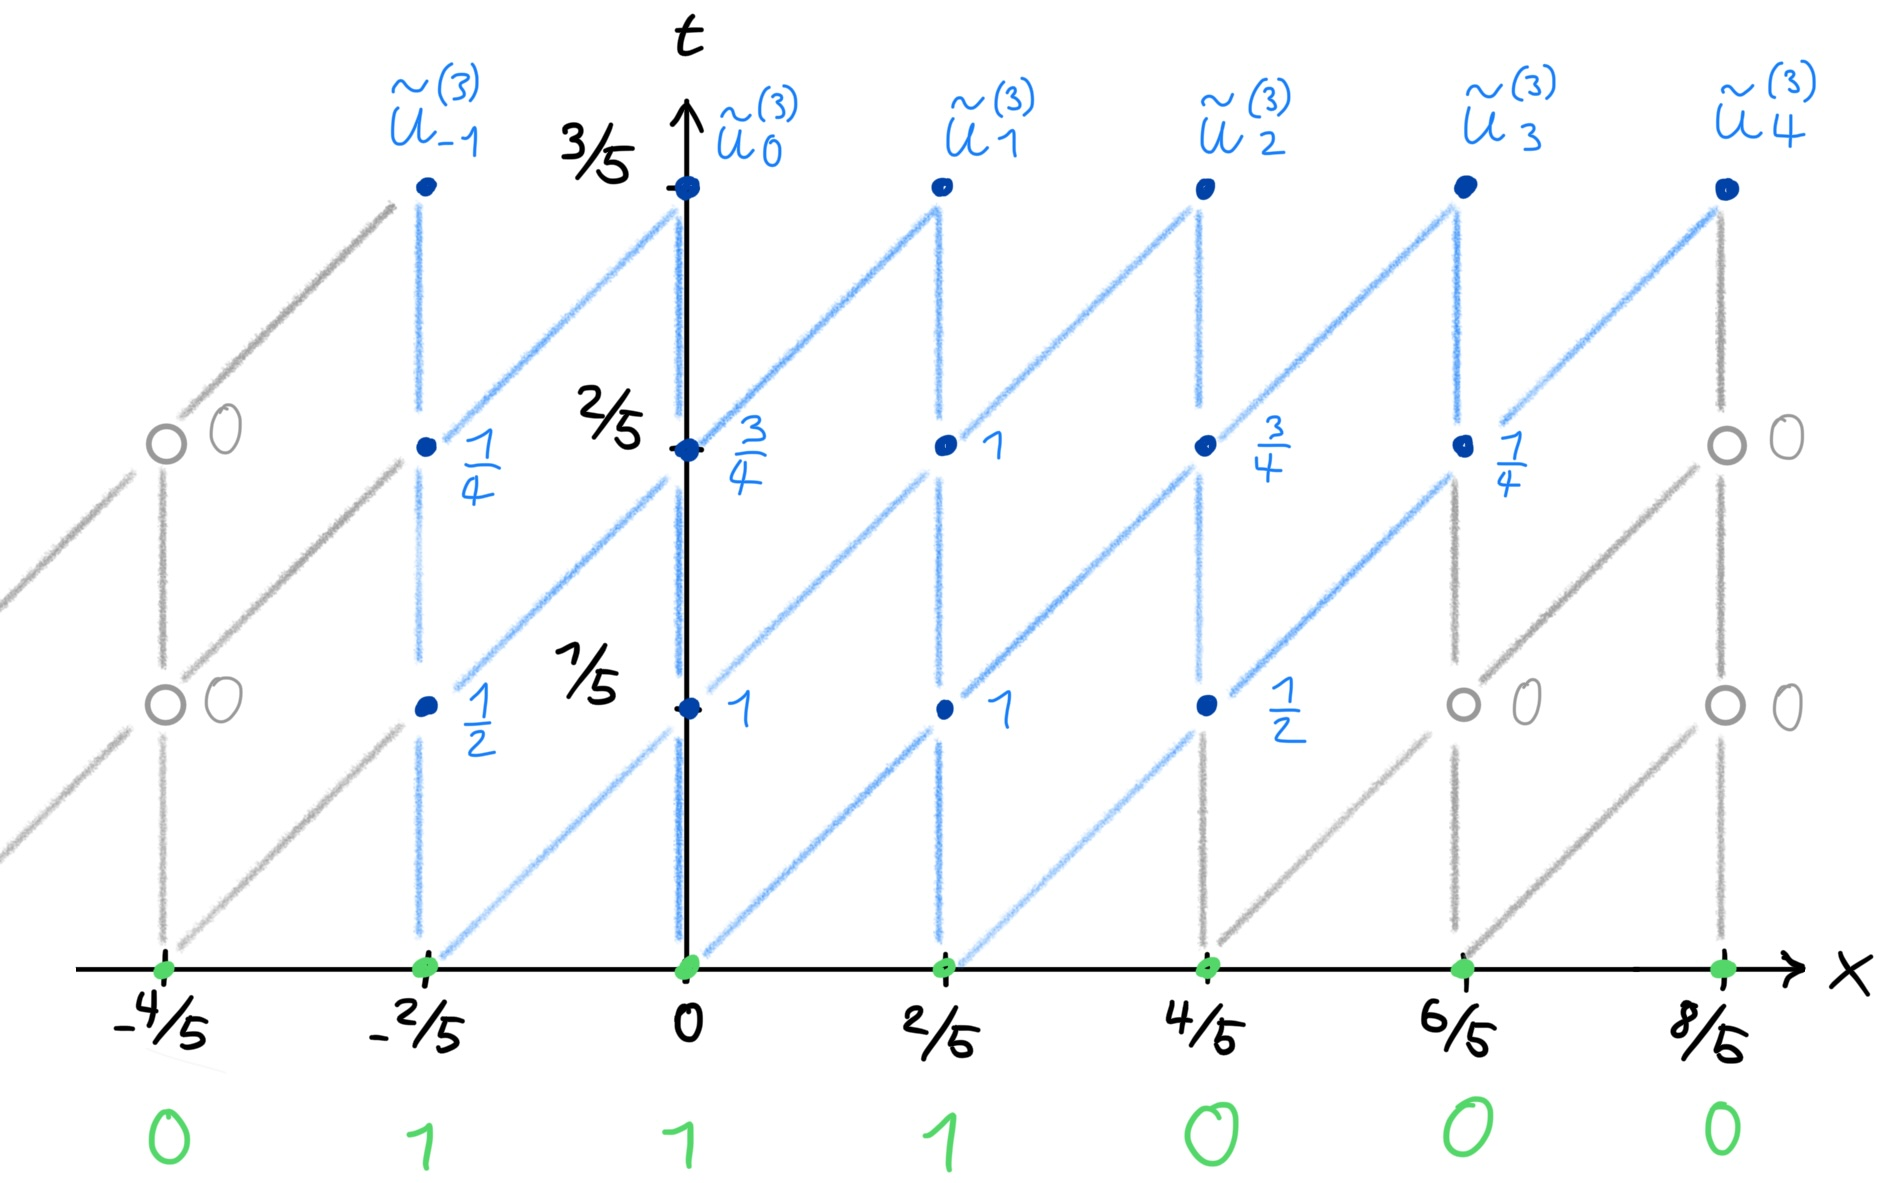
\includegraphics[width=0.8\columnwidth]{images/upwind_scheme_geometry}}
\textbf{Solution}
Using $\utild_j^{(k+1)} = \sfrac{1}{2}\cdot\utild_j^{(k)} + \sfrac{1}{2}\cdot\utild_{j-1}^{(k)}$
